\newpage
\section{Aufgabe 2}
Zur Ermittlung der Position des Moskitos wird dessen Fluggeräusch mit vier Mikrofonen gleichzeitig abgetastet.
Dabei wird das Signal mit 48kHz bzw. 96kHz abgetastet. 
Der Empfänger zeichnet gleichzeitig die empfangenen Signale an allen vier Mikrofonen auf. 
Anhand der empfangenen Signalen werden die relativen Laufzeitverzögerungen zwischen den Mikrofonen berechnet und darüber anschließend die Position mit dem bereits erklärten "Newton-Verfahren" ermittelt. Um dabei die Effizienz der Berechnung zu erhöhen, werden die von den Mikrofonen aufgezeichneten Signale gekürzt, diese gekürzten Signale bilden dabei die Hauptsignale. 
Die relativen Verzögerungen werden dadurch ermittelt, dass die Hauptsignale mit einem aus dem Hauptsignal herausgeschnittenen Teilsignal, dem Korrelationssignal, korreliert. Durch die Korrelation eines Teilsignals mit den vier Hauptsignalen lässt sich jeweils die Position des Teilsignals in den Hauptsignalen ermitteln. Anhand der Position lässt sich wiederrum die relative Verzögerung ermitteln. \\
Wie die Signale gekürzt werden, um die wichtigsten Merkmale zu erhalten und dennoch eine beringe Berechnungsdauer gewehrleisten zu können wird im folgenden geklärt.
\\ Zur Vereinfachung werden hier vorerst lediglich die Signale von zwei Mikrofonen betrachtet. 
\subsection{Herrauslösen der Hauptsignale} \label{sec:Eins}
Da die Mikrofone zeitgleich das Signal des Moskitos aufzeichnen, kommt es aufgrund der Laufzeitunterschiede des Signals zu einer Verschiebung der Signalwerte in den empfangenen Signalen untereinander. \\
So empfängt beispielsweise MIC1 den Signalabschnitt $X$ nach 10ms, wohingegen MIC2 aufgrund der größeren Entfernung zum Moskito den selben Abschnitt $X$ erst nach 20ms empfängt.\\
Beginnt man nun beim Herrauslösen der Hauptsignale am Anfang des empfangenen Signals führt dies dazu, dass Mikrofone die näher am Moskito sind diese gar nicht empfangen haben. Dies hat zur Folge, dass die Laufzeitdifferenz nicht korrekt ermittelt werden kann, da die Korrelation keine korrekten Ergebnisse liefern kann.\\
Um diesem Fehlerfall entgegenzu wirken, dürfen die Hauptsignale erst nach einem "Totbereich" herrausgelöst werden. Die Dauer des Totbereiches $t_{min}$ wird dabei über den maximal möglichen Abstand $a_{max}$ der Mikrofone zueinander ermittelt:
$$	t_{min} = \frac{a_{max}}{c_{s}} = 3.57 ms$$
Über die $t_{min}$ und die SamplingRate $f_s$ lässt sich dabei die Größe des Totbereiches $K_{min}$ in der Indexierung des Singales errechnen:
\begin{equation}
	K_{min} = f_s * t_{min}   = f_s * \frac{a_{max}}{c_{s}} \label{eq:A2A2E1}
\end{equation}

Wird der selbe pyramidenförmige Mikrofonaufbau wie im ersten Teil des Praktikums verwendet, ergibt sich für den maximalen Abstand $a_{max}$ eine Distanz von von $a_{max} = \frac{\sqrt{6}}{2}m$. Mit einer SamplingRate von $f_s = 96 kHz$ folgt aus der Gleichung\eqref{eq:A2A2E1} ein Totbereich von $K_{min} \approx 343$. Um noch etwas Sicherheit einzubauen und Rundungsfehler auszugleichen wurde für das Matlab Programm ein Totbereich von $K_{min} = 500$ gewählt.

\subsection{Herrauslösen des Korrelationssignals}
Bei dem Korrelationssignal handelt es sich um einen Auszug aus dem Hauptsignal des ersten Mikrofons welcher als Referenz für die Korrelation mit den Signalen der anderen Mikrofone benutzt wird.\\
Ähnlich wie beim Herrauslösen der Hauptsignale ist auch hier darauf zu achten, dass das Korrelationssignal in den anderen Signalen enthalten ist. Da dies allerdings bereits bei dem Herrauslösen der Hauptsignale berücksichtigt wurde, bildet der erste Teil des Hauptsignal des ersten Mikrofons das Korrelationssignal. Es wird auf eine weitere Verschiebung des Teilsignals verzichtet, um die zu bearbeitende Datenmenge so klein wie möglich zu halten.


\subsection{Länge des Korrelationssignals $K_{corr}$}
Die Länge des Korrelationssignals $K_{corr}$ beieinflusst die Genauigkeit der Differenzmessung deutlich. Ist die Länge des Teilsignals zu kurz, ist keine genaue Positionsermittlung möglich, da es sein kann, dass die betrachteten Wertfolgen mehrmals in dem Hauptsignal auftauchen, bzw. verschwimmen. Durch die Verlängerung des Teilsignals wird dies verhindert und eine exaktere Positionsbestimmung mittels der Korrelation ist möglich. Längere Zeitsignale erhöhen allerdings den Rechenaufwand und damit die Rechendauer. \\
Als Richtwert wird dabei der Extremfall mit der maximal Möglichen Signalverschiebung angewendet. Dieser tritt auf, wenn sich der Moskito auf der Verbindungsgerade der am weitesten entfernten Mikrofone und auserhalb des Raumes befindet. 
Diese maximal Mögliche Signal verschiebung wurde bereits im Unterkapitel \ref{sec:Eins}  errechnet.\\
Somit wird eine Länge des Korrelationssignals von $K_{corr}=350$ verwendet. Die Auswahl wird anhand der Simulation in Unterkapitel  \ref{sec:Untersuchung} genauer untersucht.    
\\
\subsection{Länge der Hauptsignale $K_{sig}$}
Die Länge der Hauptsignale $K_{sig}$ ist direkt von der Länge des Korrelationssignals $K_{corr}$ abhängig. Auch hier ist insbesondere der oben geschilderte Extremfall zubetrachten:\\
Da für eine möglichst exakte Bestimmung ist es notwendig, dass möglichst dass gesammte Korrelationssignal in den Hauptsignalen enthalten ist. Dies ist nur dann der Fall, wenn das Hauptsignal mindestens doppelt so lang ist wie das Korrelationssignal:
\begin{equation}
K_{sig} =  2 * K_{corr}
\end{equation}
Somit ergibt sich für das Hauptsignal eine Länge von 700 Signalwerten.
Durch die Korrelation des kürzeren Korrelationssignal mit längeren Hauptsignalen wird das Zero-Padding reduziert, wodurch eine deutlichere Bestimmung der Laufzeit unterschiede möglich ist.
\subsection{Übersicht der Signale}


\begin{figure}
\centering 
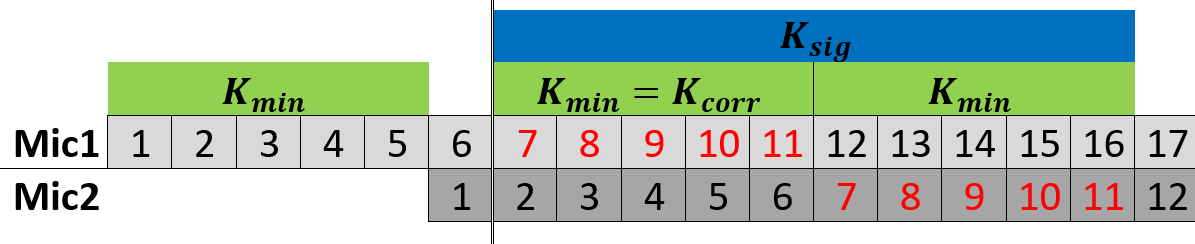
\includegraphics[width=0.4\textwidth]{Korrelation2}
\caption{Signalaufbau, anhand des Extremfalls mit maximaler Signalverschiebung}\label{fig:Korrelation2}
\end{figure}

Der Aufbau der  Signale anhand der genannten Bedingungen ist in Abbildung\ref{fig:Korrelation2} bildlich dargestellt. 
Es wird dabei der Extramfall mit einer maximalen Signalverschiebung (hier 5 ELmente) betrachtet. Würde ein Herrausschneiden der Signale (doppelte Linie) vor dem 5. Element gemacht werden, würden die entsprechenden Signale des zweiten Microfons abgeschnitten werden. Auch eine Verkürzung der Hautsignallänge (blau) würde zu einem Informaitonsverlust führen, da die Betrachtete Korrelationsfolge (rot) nicht mehr komplett im Signal2 enthalten wäre.\\
Oben beschriebene Bedingungen sind in Abbildung sind dann gültig, wenn sich das Moskito in einem Raum der nicht auf den Mikrofonraum von $1m x 1m x 1m$ begrenzt ist befinden kann.
Falls die Begrenzung auf den Mikrofonraums gilt, sollte eine Signallänge von $K_{corr}$ ausreichend sein. Bei der Begrenzung sind obige Bedingungen allerdings nicht hinderlich, sie sollten sogar zu einer höhren Genauigkeit führen. Daher wurden obige Bedinungen gewählt um den Raum des Moskitos zu erweitern.


\subsection{Untersuchung der Annahmen} \label{sec:Untersuchung}
Bei der Untersuchung der erstellten Annahmen stellte sich heraus, dass die Annahmen zu einer sehr hohen Fehlerquote bei der Korrelation führten. Ein Fehler tritt auf, wenn die über das Korrelationsmaximum ermittelte Signalverschiebung nicht mit dem tatsächlichen Wert übereinstimmt. \\

\begin{figure}
\centering 
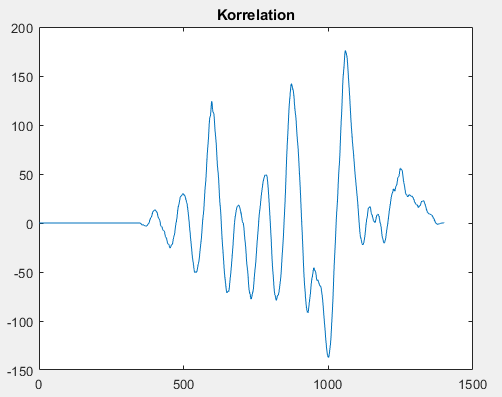
\includegraphics[width=0.4\textwidth]{KorrelationA}
\caption{Beispiel einer "fehlerhaften" Korrelation ($K_{corr}=350$}\label{fig:KorrelationA}
\end{figure}



Sieht man sich die Ergebnisse einer fehlerhaften Korrelation (siehe Abbildung \ref{fig:KorrelationA}) genauer an, fällt auf, dass kein eineindeutiges Maximum auftritt, sondern mehrere. Dabei ist das Problem, dass die "richtigen" Maxima teilweise geringere Amplituden haben als die "falschen". Dies hat zur Folge, dass eine Rechenumgebung ohne die Kenntniss der tatsächlichen Signalverschiebung teilweise falsche Ergebnisse ermitteln wird.\\
Untersucht man das Originalsignal des Moskitos (siehe Abbildung \ref{fig:KorrelationAnalyse2}) genauer fällt auf, dass das Signal eine leichte Periozität aufweist, wobei die Periodendauer des Signals ähnlich des errechneten $t_{min}$ ist. Diese Tatsache erklärt warum es bei der durchgeführten Untersuchung zu mehrern Maxima bei der Korrelation kam. \\
Zur Minimierung der Fehlerquote werden nun verschiedene Paramter untersucht

\begin{figure}
\centering 
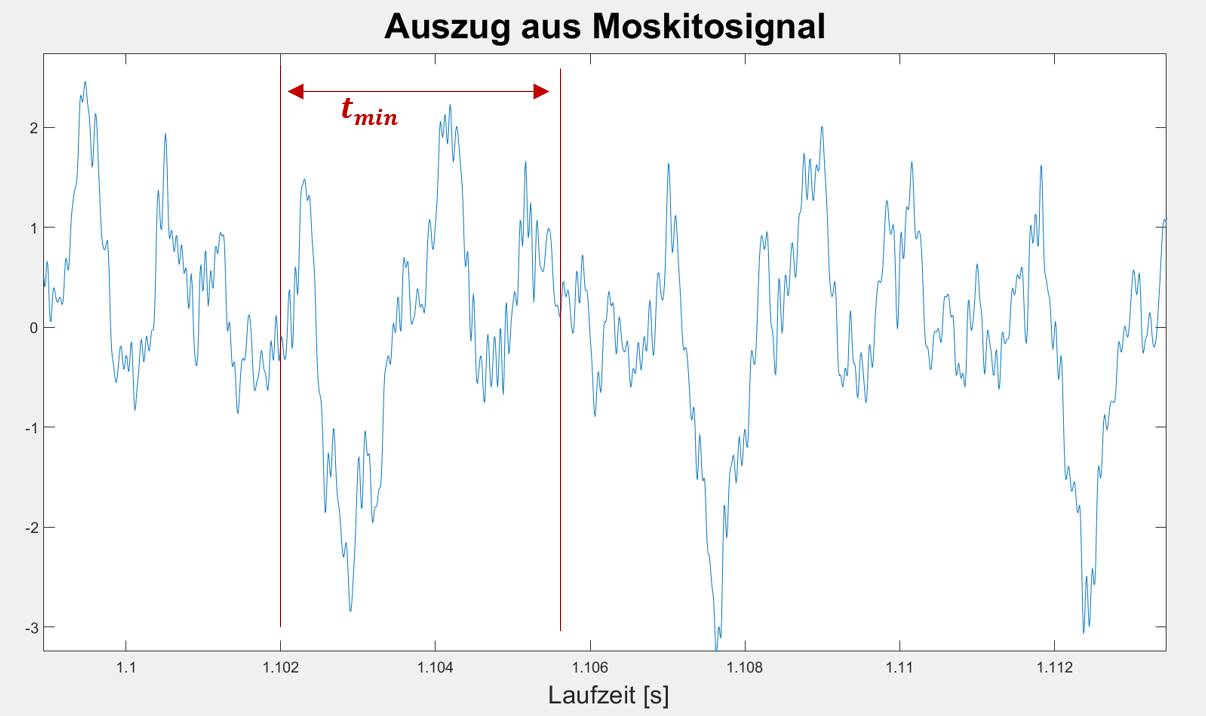
\includegraphics[width=0.4\textwidth]{KorrelationsAnalyse2}
\caption{Auszug aus dem Moskitosignal} \label{fig:KorrelationAnalyse2}
\end{figure}

\subsubsection{Länge des Korrelationssegments}

Die Betrachtung der Korrelationsergebnisse verdeutlicht, dass die errechnete Länge des Korrelationssegments zu kurz ist. Dies wurde dadurch deutlich, dass bei der Ermittlung der Korrelationswerte mehrere Maxima auftraten, da die Korrelationssegmente an mehrereren Stellen im Hauptsignal Ähnlichkeiten aufwiesen. Verlängert man das Korrelationssegment muss zwar mehr Rechenaufwand in Kauf genommen werden, allerdings nimmt auch die Wahrscheinlichkeit ab, dass man ähnliche Teile in den Hauptsignalen findet.\\


\begin{figure}
\centering 
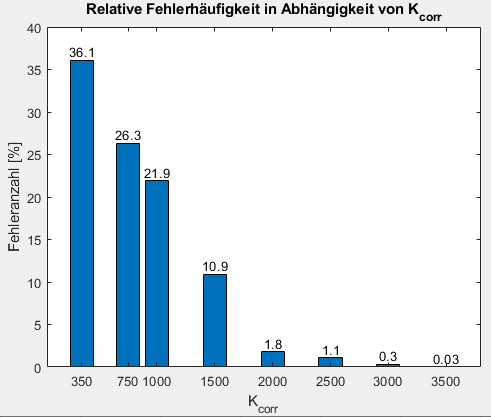
\includegraphics[width=0.4\textwidth]{KorrelationsAnalyse1}
\caption{Relative Fehlerquote in Abhängigkeit von $K_{corr}$  \linebreak(Start der Aufzeichnung nach 10000 Werten)} \label{fig:KorrelationAnalyse1}
\end{figure}

Bei der Analyse wurde die Korrelation mit allen Mikrophonen jeweils 1000 mal durchgeführt und die mittlere Fehlerquote ermittelt. Betrachtet man die Ergebnisse der Analyse (siehe Abbildung \ref{fig:KorrelationAnalyse1}) wird deutlich, dass die Fehlerquote mit zunehmender Länge von $K_{corr}$ abnimmt. Es wird deutlich, dass bei einer Korrelationslänge von 3500 Werten nur noch eine Fehlerquote von $0.03$  Prozent  erreicht wird. Mit einer weiteren Erhöhung könnte man die Fehlerquote weiter senken, allerdings würde dies die Laufzeit weiter verlängern. Betrachtet man die benötigte Laufzeit für 3500 Werte gemäß Gleichung \ref{eq:A2A2E1} wird deutlich, hierführ bereits $36.5ms$ benötigt werden.
Aufgrund des in Abbildung \ref{fig:Korrelation2} beschriebenen Signalaufbaus wird allein eine Signalmesslaufzeit von beinahe $110ms$ benötigt, wobei die benötigte Rechenzeit noch nicht berücksichtigt wurde.
Da eine noch längere Messung das Orten des Moskitos unmöglich machen, da jenes nach der Berrechnung stets an einem anderen Ort sein würde. Sollte keine größere Korrelationslänge als $K_{corr} = 3500$ gewählt  und stattdessen lieber die angegebene  Fehlerquote in Kauf genommen werden.


\subsubsection{Position des Hauptsignals}
Ein weiterer Faktor beim Signal aufbau ist der Beginn der Hauptsignale. Bei der Untersuchung dieses Parameters (siehe Abbildung \ref{fig:KorrelationAnalyse3}) sticht deutlich der Signalstart bei 7500 herraus, da dort die relative Fehlerquote am geringsten ist.
Wiederholt man nun die Analyse aus dem vorherigen Kapitel sind ist hier ebenfalls eine deutliche Verringerung der Fehlerquote zu erkennen (siehe Abbildung \ref{fig:KorrelationAnalyse4}). Auch hier wird deutlich, dass die Fehlerquote mit steigender Länge des Korrelationssignals sinkt.
\begin{figure}
\centering 
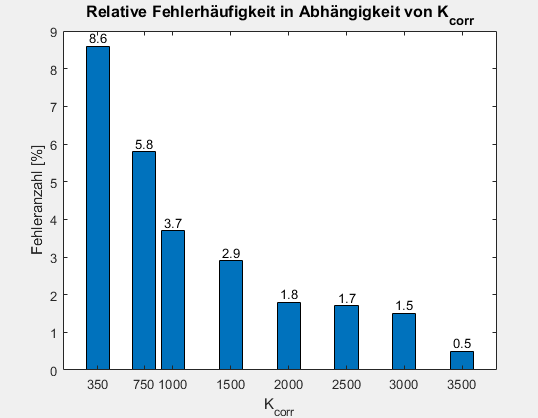
\includegraphics[width=0.4\textwidth]{KorrelationsAnalyse4}
\caption{Relative Fehlerquote in Abhängigkeit von $K_{corr}$  \linebreak(Start der Aufzeichnung nach 7500 Werten)} \label{fig:KorrelationAnalyse4}
\end{figure}

\begin{figure}
\centering 
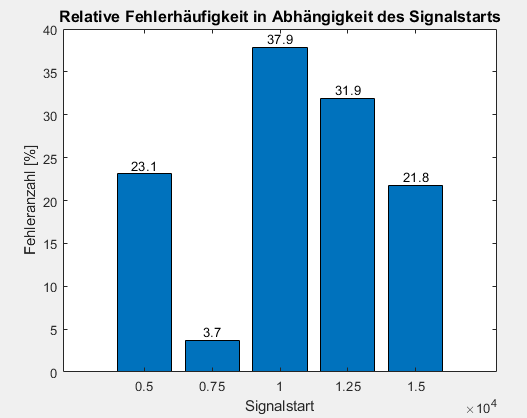
\includegraphics[width=0.4\textwidth]{KorrelationsAnalyse3}
\caption{Relative Fehlerquote in des Signalstarts $K_{corr}$  \linebreak(5000 Messungen mit $K_{corr}=1000$)} \label{fig:KorrelationAnalyse3}
\end{figure}
\subsubsection{Zusammenfassung der Untersuchung }
Abschließend lässt sich zusammenfassen, dass die berechenete Länge des Korrelationssignal deutlich zu kurz für eine akzeptable Positionsbestimmung ist. Aus der Analyse des Startwartes wird deutlich, dass die Ergebnisse stark von dem jeweiligen Signalabschnitt abhängen. Da es in der Realität das Signal des Moskitos allerdings nicht statisch ist wie in der Simulation, ist diese Analyse sekundär, da die Position beim realen Signal nicht beeinflusst werden kann. Allerdings lässt diese Position gut für die Analyse des Rauscheinflusses verwenden. \\\\\\
Für weitere Berechnungen werden von nun an die Parameter wie folgt gewählt:\\
$$K_{Startwert} = 7500$$
$$K_{corr} = 3000$$
$$K_{sig} = 6000$$

\subsubsection{Korrelation mit awgn Rauschen }
Bis jetzt haben wir angenommen, dass das Audiosignal auf dem Weg von der Signalquelle zum Mikrophon nicht gestört wird. Nun betrachten wir den Fall mit Rauschen. Wir gehen davon aus, dass wir ein Additive White Gausian Noise (awgn) haben. Dabei handelt es sich um ein Normalverteiltes Zufallssignal mit unendlicher Bandbreite, welches auf unser Nutzsignal aufaddiert wird. Dabei ist das Rauschen auf dem Weg zu Mikrofon 1 unabhängig vom Rauschen auf dem Weg zu Mikrofon 2. Wir wollen nun untersuchen wie dieses Rauschen unser Korrelationsergebnis beeinflusst. Wichtig hierbei ist das Signal to Noise Ratio. Dies beschreibt das Verhältnis der Leistungen vom Nutzsignal zum Rauschsignal. 
$$ snr = \frac{P_{nutzsignl}}{P_{Rauschsignal}} [dB]$$
Mit Hilfe eines Matlab Scripts haben wir simuliert wie sich awgn Rauschen auf die Korrelation auswirkt. Wir haben die Korrelation jeweils 1000 mal für unterschiedliche snr durchlaufen lassen. Die Position der Signalquelle war jedes mal zufällig. Auf dem Schaubild (siehe Abbildung \ref{fig:KorrelationAnalyseMitRauschen}) ist zu sehen, dass wir bis zu einem snr von 7dB eine Fehlerquote von 0\% haben. Bei einem snr von 0dB bzw. 1/1 haben wir gerade einmal eine Fehlerquote von 3\%.


\begin{figure}
\centering 
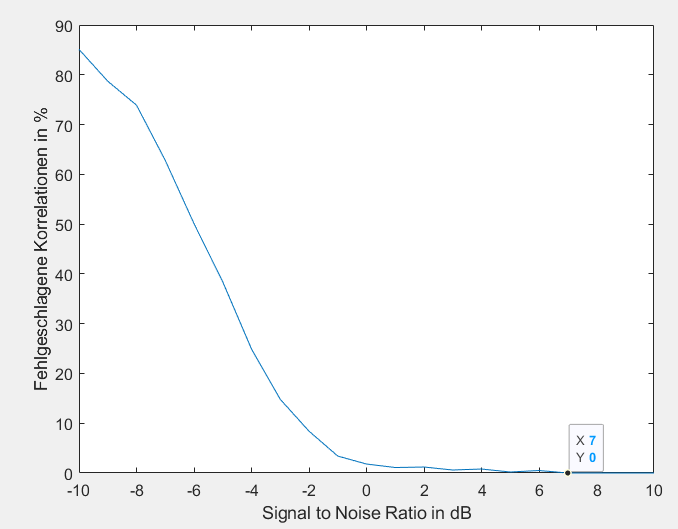
\includegraphics[width=0.4\textwidth]{Correlation mit Rauschen, (SNR) bei 4000 Segmentlaenge und 7500 corrBegin (in dB)}
\caption{Korrelation mit Rauschen} \label{fig:KorrelationAnalyseMitRauschen}
\end{figure}